\begin{frame}[fragile]
	\frametitle{The Kernel of \cuda}
	\cuda{} is an extension of C/C++ which allows for \emph{kernels}, functions executed $N$ times in parallel by $N$ different \cuda{} threads.
	\begin{columns}
		\begin{column}{.68\columnwidth}
\begin{lstlisting}
// Kernel definition by means 
// of __global__ keyword
__global__
void VecAdd(float* A, float* B,
            float* C) {
	int i = threadIdx.x;
	C[i] = A[i] + B[i];
}

int main() {
	...
	// Kernel <1 block, N threads> 
	VecAdd<<<1, N>>>(A, B, C);
	...
}
\end{lstlisting}
		\end{column}

		\begin{column}{.32\columnwidth}
			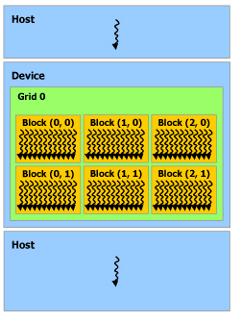
\includegraphics[
				%height=\textheight
				width=1.\columnwidth
				]{fig/heterogeneous-programming_CUT.jpg}
		\end{column}
	\end{columns}

\end{frame}
